\documentclass{beamer}
\usetheme[faculty=econ]{fibeamer}

\usepackage[utf8]{inputenc}
\usepackage[francais]{babel}
\usepackage[T1]{fontenc}
\usepackage{xcolor}

\lstset{
  language=Java,                
  basicstyle=\scriptsize,
  escapeinside={*@}{*@},
  frame=single,
  xleftmargin=2mm,
  xrightmargin=2mm,
  keepspaces=true,
  tabsize=2
}

\newcounter{ctr1}
\title[]{\Large{Développement d'applications modulaires en Java}}
\author[C. Tibermacine]{\large{Chouki~Tibermacine}\\
\small{Chouki.Tibermacine@umontpellier.fr}}
%\institute{Polytech Montpellier}
\date{}

\begin{document}

\begin{frame}
\titlepage
\begin{flushright}

\includegraphics[width=3.5cm]{figs/polytech.png}
\end{flushright}
\end{frame}

\begin{frame}
	\frametitle{Plan de l'ECUE}
	\begin{enumerate}
		{\color{gray}{\item (Rappels sur le) Développement d'applications Web avec Java
				\item Modulariser les applications Java avec Spring
				\item Bien structurer une application Web avec Spring MVC
				\item Auto-configurer une application Web avec Spring Boot
				\item Sécuriser une application Web avec Spring Security}}
				\item Gérer des données massives avec Apache Kafka et Spring
		{\color{gray}{				\item Tester une application Web Spring
				\item Écrire des applications Web (API) réactives avec Spring WebFlux}}
	\end{enumerate}
\end{frame}

\AtBeginSection[]{% Print an outline at the beginning of sections
  \begin{frame}<beamer>
    \frametitle{Plan du cours}
    % \frametitle{Outline}
    \tableofcontents[currentsection]
    % \tableofcontents
  \end{frame}}

\AtBeginSubsection[]{% Print an outline at the beginning of sections
  \begin{frame}<beamer>
    \frametitle{Plan du cours}
    % \frametitle{Outline}
    \tableofcontents[currentsubsection]
    % \tableofcontents
  \end{frame}}

\section{Introduction à Apache Kafka}

\begin{frame}
  \frametitle{Qu'est-ce que ``\textit{Apache Kafka}''}
	\begin{tikzpicture}[overlay,remember picture]
	\node[anchor=center,xshift=0pt,yshift=-20pt]
	at (current page.center) {
		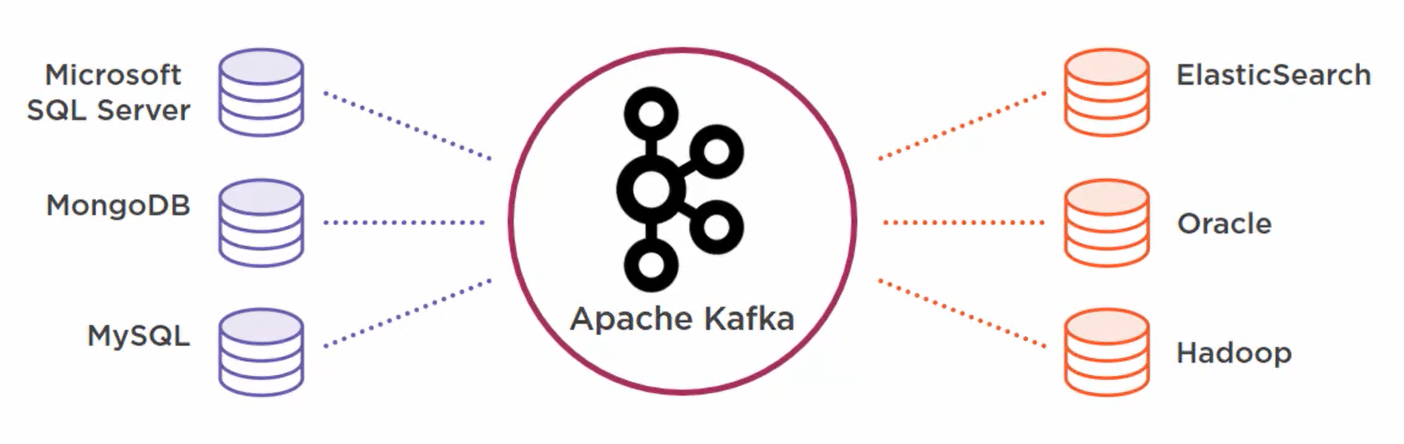
\includegraphics[width=12cm]{img/intro_kafka.png}
	};
	\end{tikzpicture}
\begin{center}
Un système distribué de messagerie publish/subscribe \\
  à grand débit
  \vspace{5cm}

\end{center}
\end{frame}

\begin{frame}
	\frametitle{Particularités de Kafka}
	\begin{itemize}
		\item Spécialement conçu pour un grand débit de messages (des centaines de millions d'utilisateurs et des milliers de milliards de messages par jour)
		\item A prouvé son efficacité chez LinkedIn, Netflix, Uber, Airbnb, ...
		\item Garantit une certaine fiabilité en répliquant les messages
		\item Traditionnellement, on utilisait la réplication de bases de données, mais c'est peu flexible (la migration d'un fournisseur (\textit{vendor}) à un autre ou une évolution des schémas posent des problèmes, parfois complexes)
		\item Utilisable pour l'interopérabilité entre des sources de données hétérogènes
	\end{itemize}
\end{frame} 

\begin{frame}
	\frametitle{Un courtier (\textit{broker}) de messages}
	\begin{tikzpicture}[overlay,remember picture]
		\node[anchor=east,xshift=0pt,yshift=-20pt]
		at (current page.east) {
			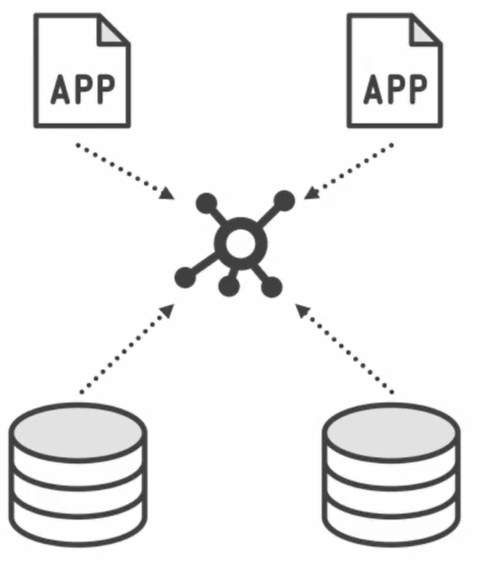
\includegraphics[width=5cm]{img/message_broker.png}
		};
	\end{tikzpicture}
	\begin{itemize}
		\item Permettant de découpler les producteurs\\
		 et les consommateurs de messages
		\item Basé sur le pattern publish/subscribe
		\item Messages durables ou effaçables
	\end{itemize}
\end{frame} 

\begin{frame}
	\frametitle{LinkedIn avant 2010}
	\begin{tikzpicture}[overlay,remember picture]
		\node[anchor=center,xshift=0pt,yshift=-20pt]
		at (current page.center) {
			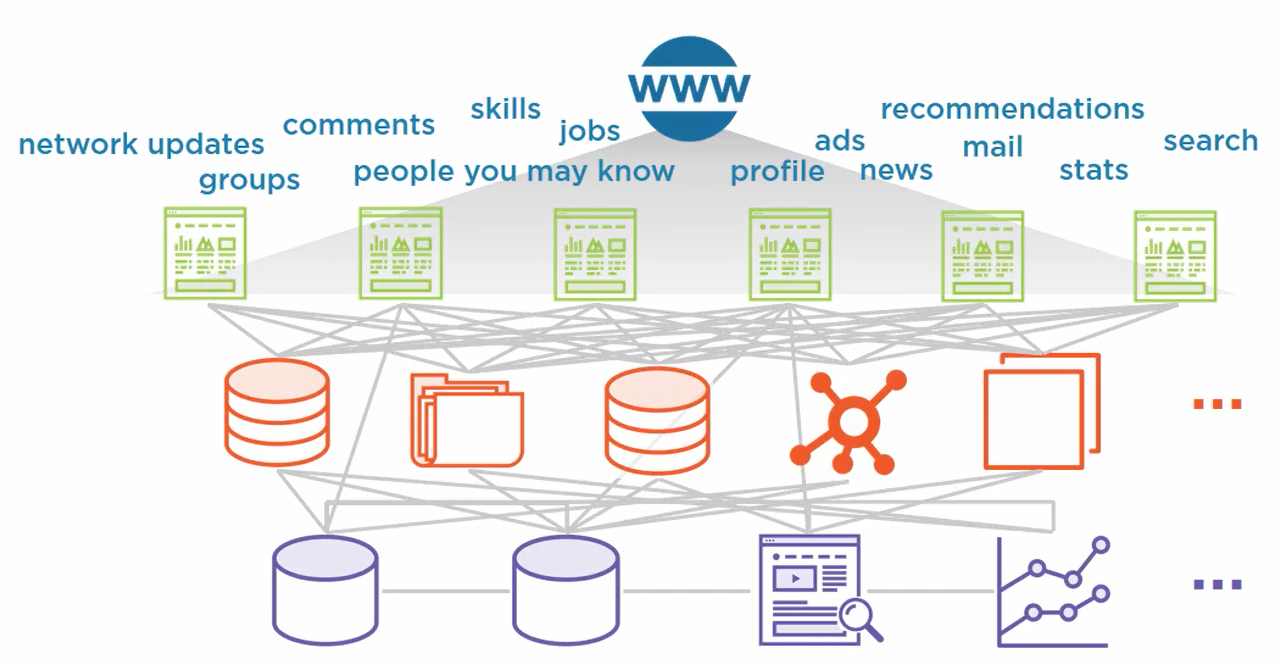
\includegraphics[width=12cm]{img/linkedin_before.png}
		};
	\end{tikzpicture}
\end{frame} 

\begin{frame}
	\frametitle{LinkedIn après 2010}
	\begin{tikzpicture}[overlay,remember picture]
		\node[anchor=center,xshift=0pt,yshift=-20pt]
		at (current page.center) {
			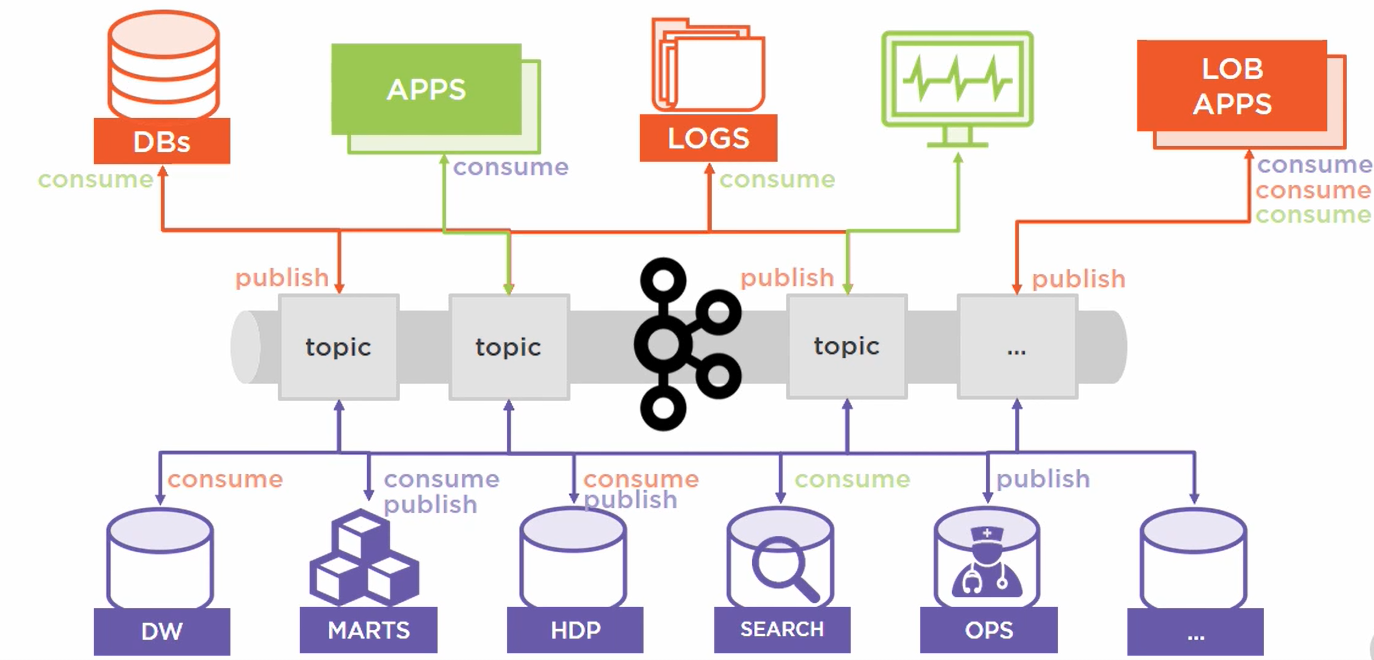
\includegraphics[width=12cm]{img/linkedin_after.png}
		};
	\end{tikzpicture}
\end{frame} 

\begin{frame}
	\frametitle{LinkedIn et Kafka}
\begin{itemize}
	\item LinkedIn existe depuis 2003
	\item Début du développement de Kafka en 2009
	\item En 2010, c'est opérationnel chez LinkedIn
	\item En 2011/2012, Kafka est devenu un projet open-source Apache (l'un des plus utilisés de la fondation)
	\item Aujourd'hui, LinkedIn gère 1.1 k milliards de messages / jour avec Kafka
\end{itemize}
	
\end{frame} 

\begin{frame}
	\frametitle{Producers (publishers), Consumers (subscribers) \& Topics}
	\begin{tikzpicture}[overlay,remember picture]
		\node[anchor=center,xshift=0pt,yshift=-20pt]
		at (current page.center) {
			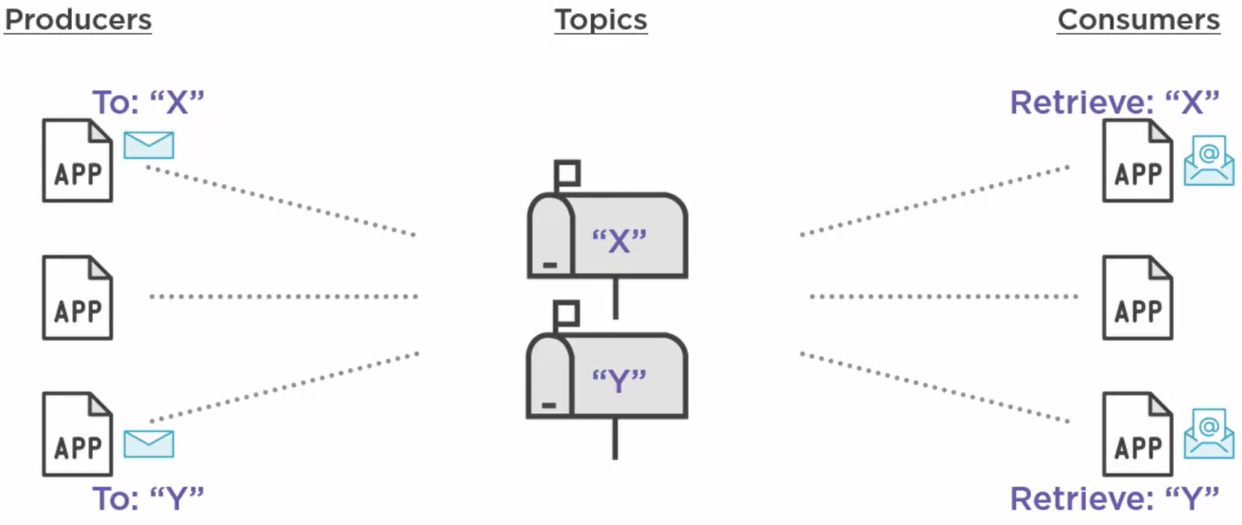
\includegraphics[width=12cm]{img/prod_cons_topic.png}
		};
	\end{tikzpicture}
\begin{itemize}
	\vspace{5cm}
	\item[] Topics = groupes de messages
\end{itemize}
\end{frame} 

\begin{frame}
	\frametitle{Courtiers ou \textit{brokers}}
	\begin{tikzpicture}[overlay,remember picture]
		\node[anchor=center,xshift=0pt,yshift=0pt]
		at (current page.center) {
			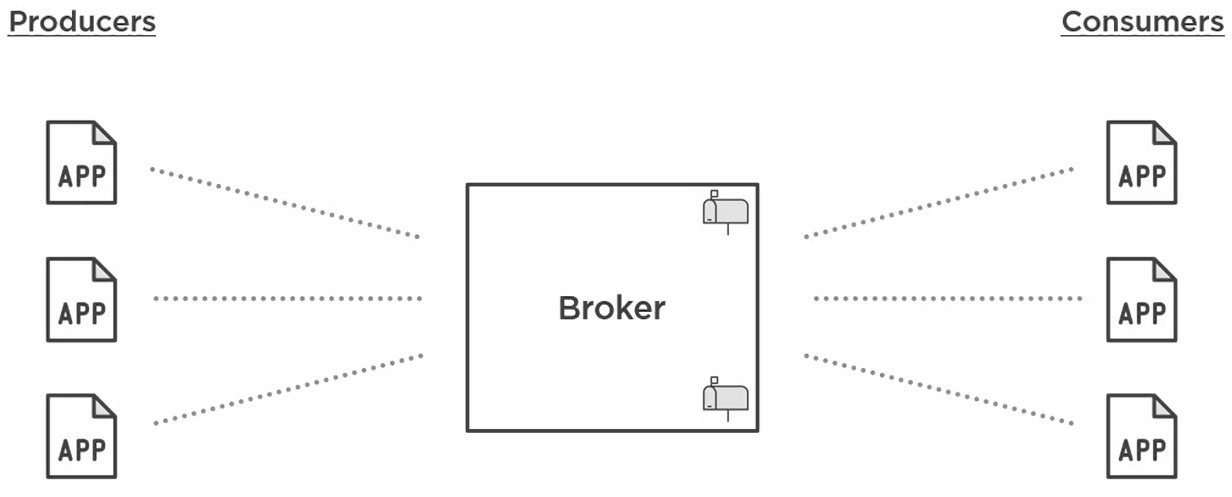
\includegraphics[width=12cm]{img/broker.png}
		};
	\end{tikzpicture}
	\begin{itemize}
		\vspace{5cm}
		\item Borker : gère un ensemble de topics
		\item C'est un processus (deamon) serveur
	\end{itemize}
\end{frame} 

\begin{frame}
	\frametitle{On peut créer un nombre quelconque de \textit{brokers}}
	\begin{tikzpicture}[overlay,remember picture]
		\node[anchor=center,xshift=0pt,yshift=20pt]
		at (current page.center) {
			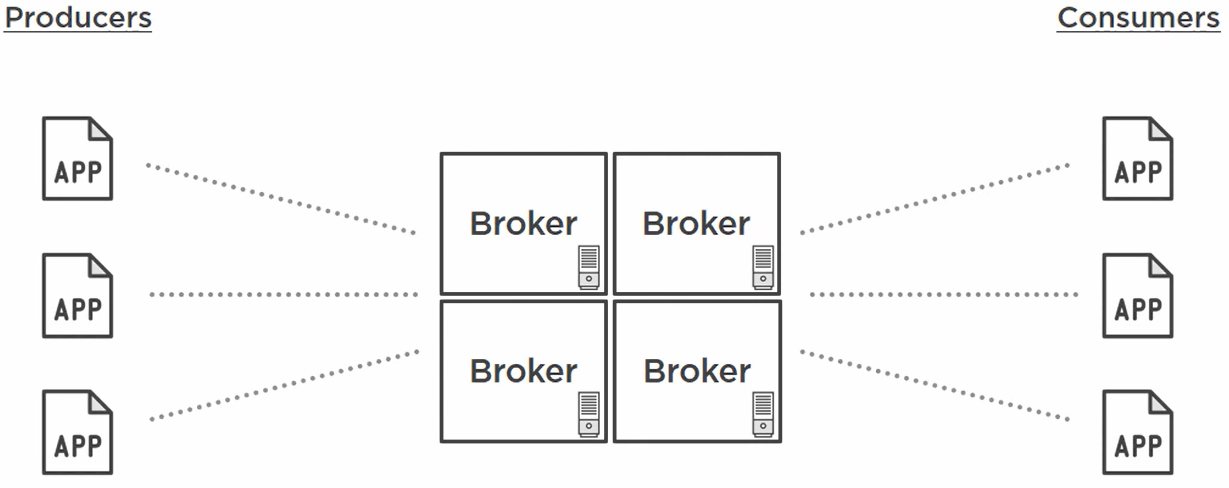
\includegraphics[width=12cm]{img/multi_broker.png}
		};
	\end{tikzpicture}
	\begin{itemize}
		\vspace{4.5cm}
		\item C'est ce qui permet de gérer les gros débits de messages
		\item En 10.2019, LinkedIn a déclaré utiliser 4000 brokers avec 100 000 topics pour 7k millairds de messages par jour~:\\
		\footnotesize
		\url{https://engineering.linkedin.com/blog/2019/apache-kafka-trillion-messages}
		\normalsize
	\end{itemize}
\end{frame} 

\begin{frame}
	\frametitle{Cluster}
	\begin{tikzpicture}[overlay,remember picture]
		\node[anchor=center,xshift=0pt,yshift=0pt]
		at (current page.center) {
			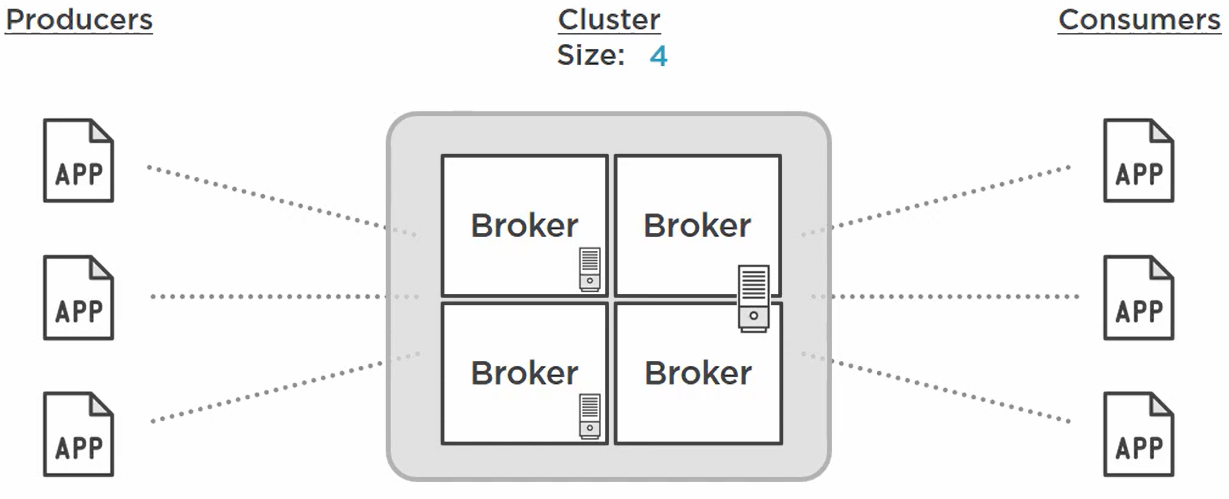
\includegraphics[width=12cm]{img/cluster.png}
		};
	\end{tikzpicture}
	\begin{itemize}
		\vspace{5cm}
		\item Cluster : ensemble de brokers
	\end{itemize}
\end{frame} 

\begin{frame}
	\frametitle{Apache Zookeeper}
	\begin{tikzpicture}[overlay,remember picture]
		\node[anchor=center,xshift=0pt,yshift=15pt]
		at (current page.center) {
			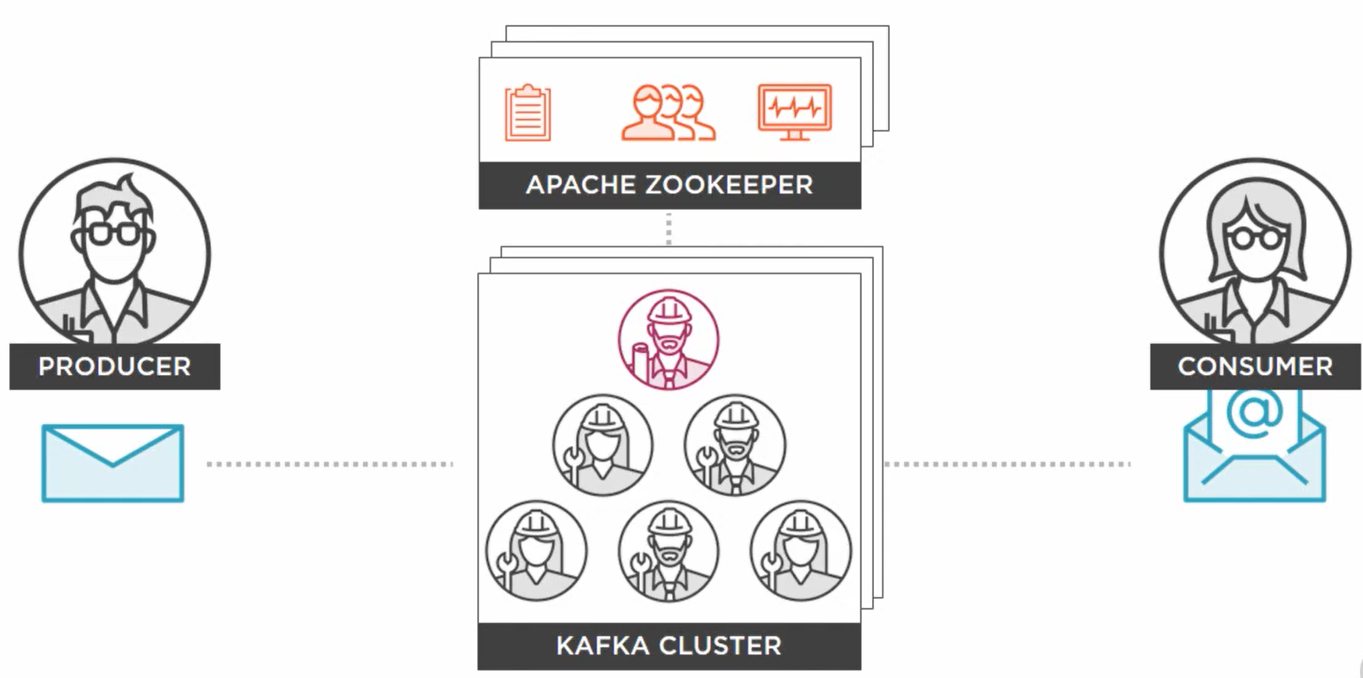
\includegraphics[width=11cm]{img/zookeeper.png}
		};
	\end{tikzpicture}
	\begin{itemize}
		\vspace{5cm}
		\item Un système distribué (serveur) pour gérer les méta-données (état de santé, config, ...) sur les clusters
		\item C'est lui qui choisit quel broker est responsable de quel topic
		\item Utilisé dans d'autres projets aussi (Hadoop, Redis, Neo4j, ...)
	\end{itemize}
\end{frame} 

\begin{frame}
	\frametitle{Une intro différente à Kafka}
	\begin{itemize}
		\item \url{https://www.youtube.com/watch?v=FKgi3n-FyNU}
	\end{itemize}
\end{frame} 


\section{Topics, Partitions et Brokers}

\begin{frame}
	\frametitle{Installer Kafka à la main}
	\begin{itemize}
		\item Ouvrir un terminal
		\item Installer Scala si vous ne l'avez pas (une partie de Kafka a été écrite avec Scala)~:
		\footnotesize
		\texttt{sudo apt install scala} (sous Linux)
		\normalsize
		\item Télécharger l'archive qui se trouve ici :\\
		\footnotesize
		\texttt{wget https://mirrors.ircam.fr/pub/apache/kafka/3.0.0/kafka\_2.12-3.0.0.tgz}\\
		\normalsize
		Mettre à jour l'URL s'il y a une version plus récente
		\item Décompresser l'archive :\\
		\texttt{tar xvzf kafka\_2.12-2.6.0.tgz}
		\item Explorer le dossier, qui a une structure classique~: \texttt{bin/} (scripts Shell + un dossier \texttt{windows/} avec les scripts Batch), \texttt{config/}, \texttt{libs/}, ...
	\end{itemize}
\end{frame} 

\begin{frame}
	\frametitle{Topics}
	\begin{tikzpicture}[overlay,remember picture]
		\node[anchor=north,xshift=90pt,yshift=0pt]
		at (current page.north) {
			
\includegraphics[width=3cm]{img/topic.png}
		};
	\end{tikzpicture}
	\begin{itemize}
		\item Une abstraction (entité logique) au cœur du système
		\item Une catégorie ou un flux nommé de messages
		\item Les producteurs produisent des messages dans un topic
		\item Les consommateurs consomment des messages depuis un topic
		\item Physiquement représentés comme fichiers logs (Kafka = \textit{distributed commit log})
	\end{itemize}
\end{frame} 

\begin{frame}
	\frametitle{Topic : entité vue par les prod. \& conso.}
	\begin{tikzpicture}[overlay,remember picture]
		\node[anchor=center,xshift=0pt,yshift=10pt]
		at (current page.center) {
			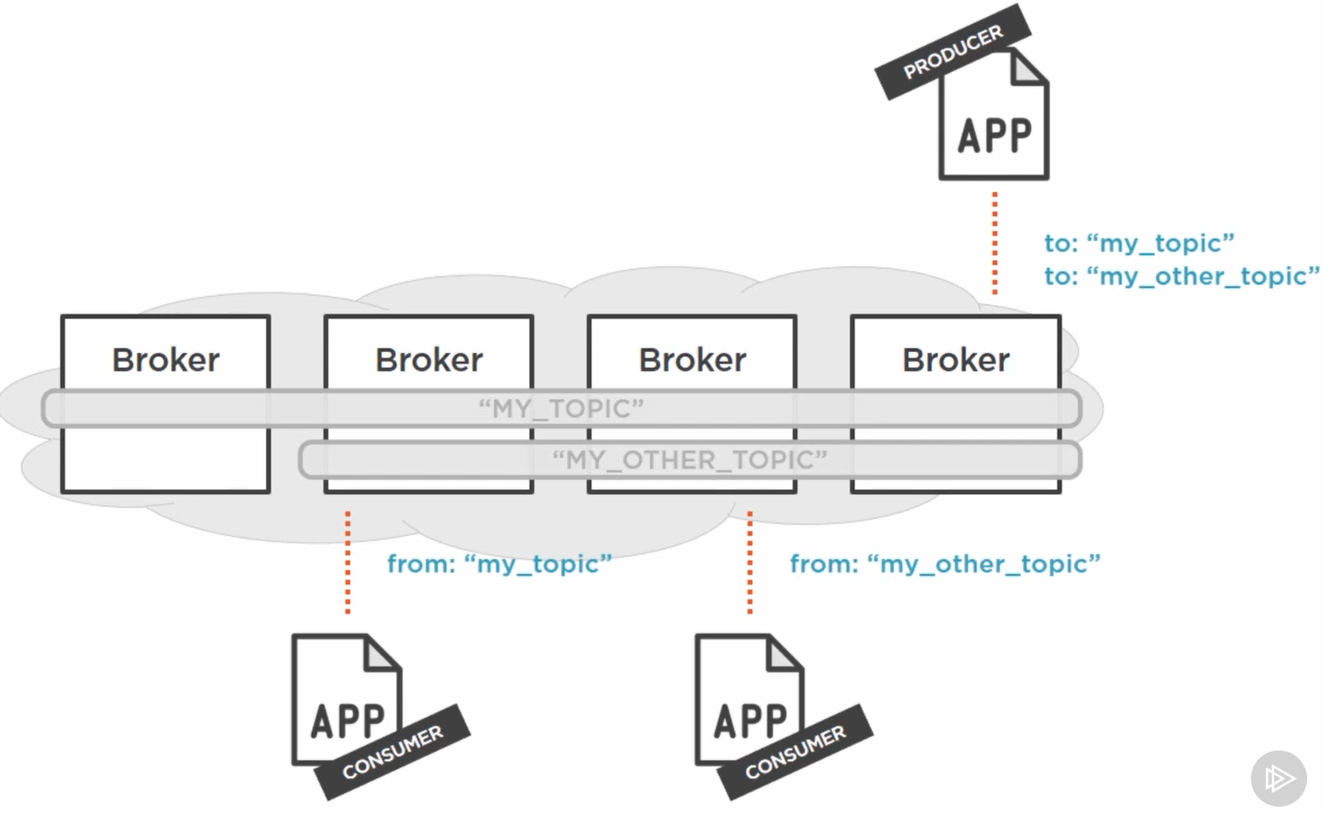
\includegraphics[width=9cm]{img/topics_over_brokers.png}
		};
	\end{tikzpicture}
	\begin{itemize}
		\vspace{5cm}
		\item Topics sur plusieurs brokers pour la fiabilité
		\item Mais les producteurs et consommateurs voient des topics (peu importe leur emplacement)
	\end{itemize}
\end{frame} 

\begin{frame}
	\frametitle{Topic : une séquence ordonnée}
	\begin{tikzpicture}[overlay,remember picture]
		\node[anchor=center,xshift=0pt,yshift=25pt]
		at (current page.center) {
			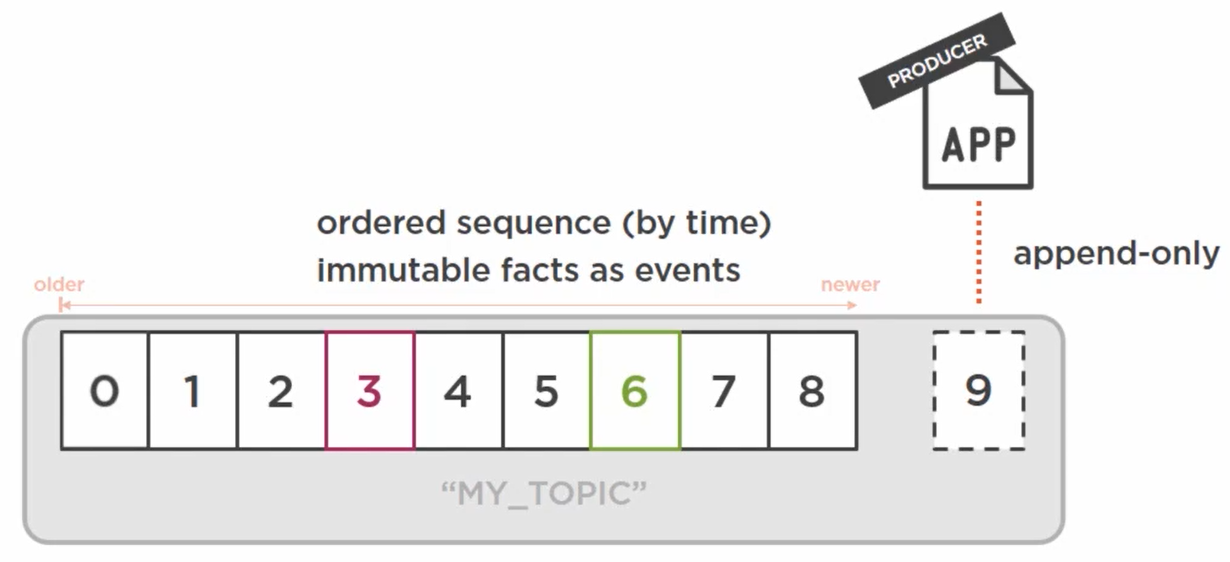
\includegraphics[width=10cm]{img/topic_file_messages.png}
		};
	\end{tikzpicture}
	\begin{itemize}
		\vspace{4cm}
		\item Topic = séquence ordonnée par le temps
		\item Messages = événements (enregistrements ou \textit{records}) immuables (système fonctionnant selon le style \textit{Event Sourcing})
		\item Messages insérés à la fin du topic et horodatés
		\item Au consommateur de repérer l'évolution d'un message (producteur incapable de changer un message existant)
	\end{itemize}
\end{frame} 

\begin{frame}
	\frametitle{Message}
	\begin{tikzpicture}[overlay,remember picture]
		\node[anchor=east,xshift=0pt,yshift=30pt]
		at (current page.east) {
			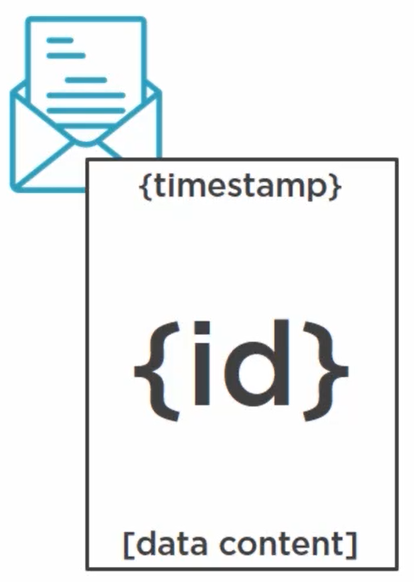
\includegraphics[width=3cm]{img/message.png}
		};
	\end{tikzpicture}
Chaque message~:
	\begin{enumerate}
		\item est horodaté (a un \textit{timestamp})
		\item a un identifiant unique utilisé par les producteurs\\ et les consommateurs
		\item[] La paire (timestamp,identifiant) est unique
		\item a un contenu (\textit{payload}) binaire
	\end{enumerate}
\vspace{1cm}
La défaillance d'un consommateur n'a aucun impact sur les messages, les autres consommateurs ou les producteurs
\end{frame} 

\begin{frame}
	\frametitle{Offset}
	\begin{tikzpicture}[overlay,remember picture]
		\node[anchor=center,xshift=0pt,yshift=40pt]
		at (current page.center) {
			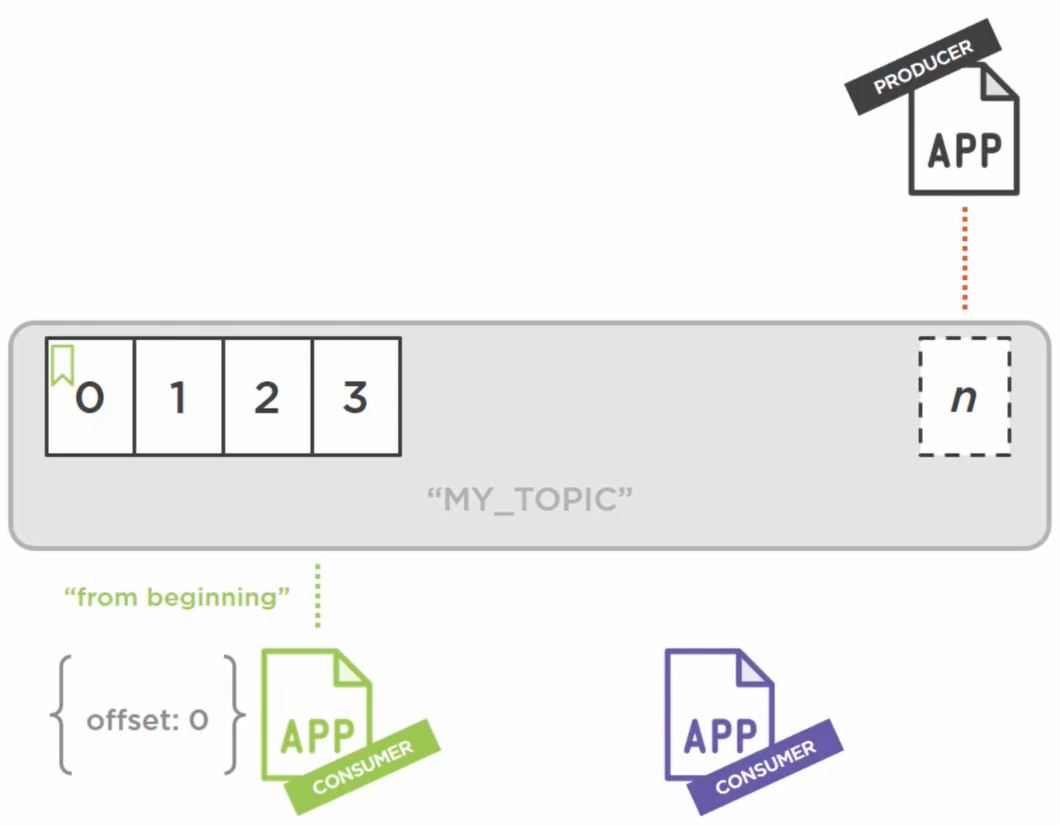
\includegraphics[width=8cm]{img/offset.png}
		};
	\end{tikzpicture}
	\begin{itemize}
		\vspace{4cm}
		\item Une sorte de marque-page qui correspond à la position du dernier message consommé
		\item Chaque consommateur peut évoluer indépendamment des autres dans la consommation des messages
	\end{itemize}
\end{frame}

\begin{frame}
	\frametitle{Politique de rétention des messages}
	\begin{itemize}
		\item Kafka garde tous les messages produits, qu'ils soient consommés ou pas
		\item La durée de rétention des messages est configurable en heures
		\item Par défaut, la durée de rétention est de 168 heures (7 jours)
		\item La période de rétention est définie par topic
		\item Le stockage physique peut contraindre la durée de rétention
	\end{itemize}
\end{frame} 

\begin{frame}
	\frametitle{Démo à faire, en ligne de commande}
	\begin{enumerate}
		\item Démarrer un serveur Zookeeper~:\\
		\footnotesize
		\texttt{bin/zookeeper-server-start.sh config/zookeeper.properties}\\
		* Un processus serveur est démarré sur le port 2181
		\normalsize
		\item Démarrer un broker~:\\
		\footnotesize
		\texttt{bin/kafka-server-start.sh config/server.properties}\\
		* Un processus serveur est démarré sur le port 9092
		\normalsize
		\item Créer un topic~:\\
		\footnotesize
		\texttt{bin/kafka-topics.sh ---create ---topic my\_topic ---zookeeper <votre-hostname>:2181 ---replication-factor 1 ---partitions 1}\\
		\normalsize
		Pour obtenir le hostname, taper la commande \texttt{hostname} sur un terminal
		\item Lister les topics~:\\
		\footnotesize
		\texttt{bin/kafka-topics.sh ---list ---zookeeper <votre-hostname>:2181}
		\normalsize
	\end{enumerate}

\end{frame} 
		
\begin{frame}
	\frametitle{Démo à faire, en ligne de commande -suite-}
	\begin{enumerate}		
		\item Produire un message~:\\
		\footnotesize
		\texttt{bin/kafka-console-producer.sh ---broker-list <votre-hostname>:9092 ---topic my\_topic}\\
		\normalsize		
		Ceci permet d'obtenir un Shell dans lequel on peut écrire plusieurs messages, séparés par des validations sur la touche ``Entrée''
		\item Consommer un message~:\\
		\footnotesize
		\texttt{bin/kafka-console-consumer.sh ---bootstrap-server <votre-hostname>:9092 ---topic my\_topic ---from-beginning}\\
		\normalsize		
		Les anciens messages s'affichent et chaque nouveau message produit par un producteur va apparaître
	\end{enumerate}
Pour supprimer un topic~:\\
\footnotesize 
\texttt{bin/kafka-topics.sh ---delete ---zookeeper <votre-hostname>:2181 ---topic my\_topic}
\normalsize
\end{frame} 

\begin{frame}
	\frametitle{Partitions Kafka}
	\begin{tikzpicture}[overlay,remember picture]
		\node[anchor=east,xshift=0pt,yshift=-10pt]
		at (current page.east) {
			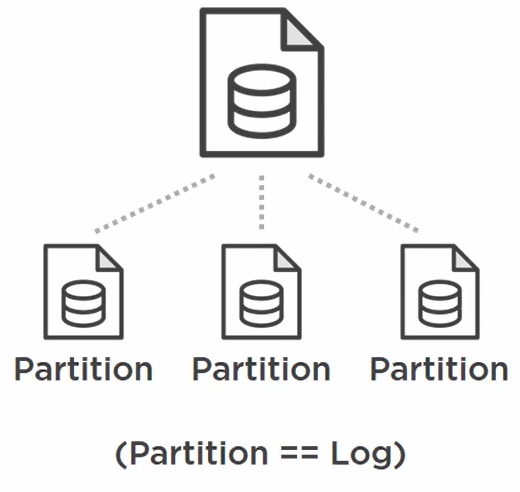
\includegraphics[width=4cm]{img/partition.png}
		};
	\end{tikzpicture}
	\begin{itemize}
		\item Une partition = un log physique (fichiers)
		\item Un topic a une ou +ieurs partitions
		\item Une partition est la base pour Kafka\\ pour gérer la scalabilité, la tolérance\\ aux fautes et la gestion d'un gros débit
		\item Chaque partition est maintenue\\
		sur au moins un broker
		\item Dans l'exemple précédent, nous avons créé\\ un topic avec une seule partition (\texttt{---partitions 1})
	\end{itemize}
\end{frame} 

\begin{frame}
	\frametitle{Une partition sur une machine}
	\begin{tikzpicture}[overlay,remember picture]
		\node[anchor=center,xshift=0pt,yshift=20pt]
		at (current page.center) {
			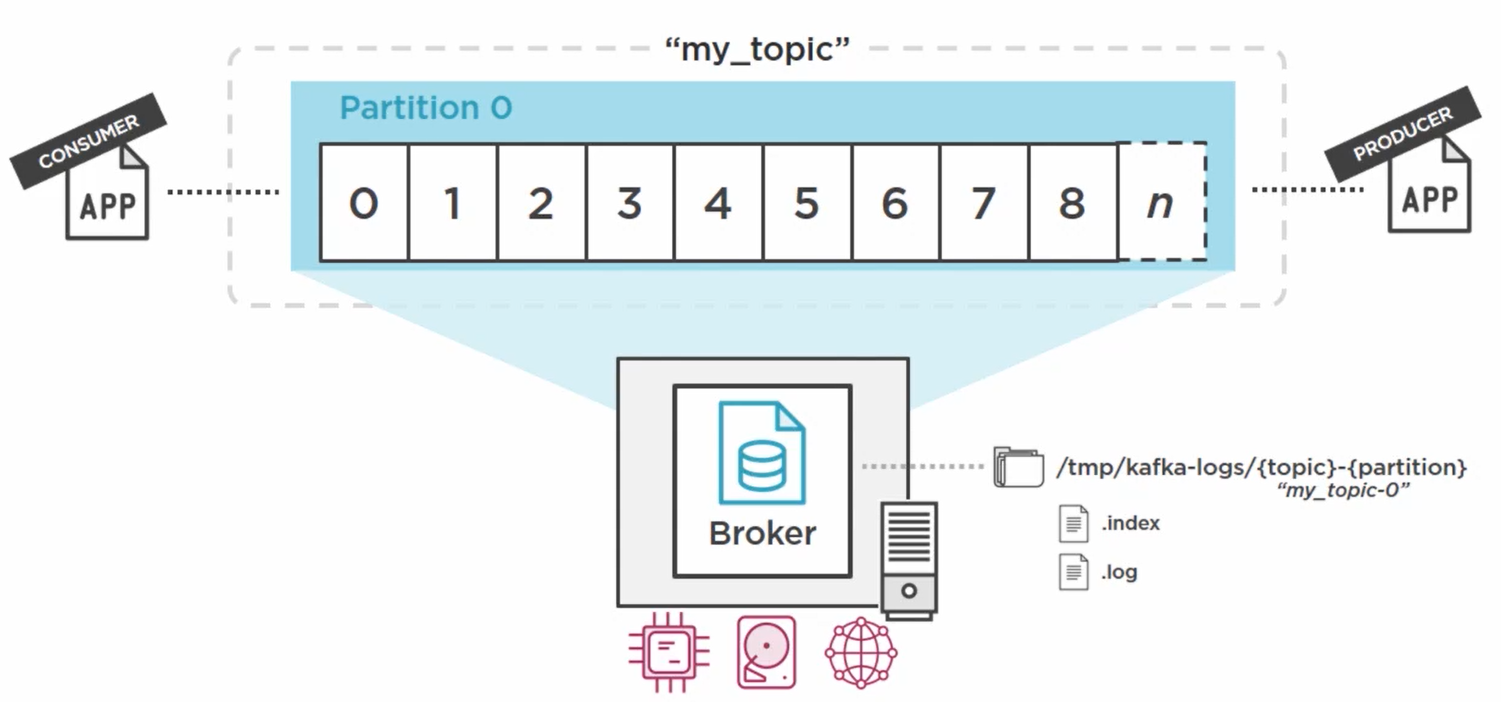
\includegraphics[width=10cm]{img/partition_disk.png}
		};
	\end{tikzpicture}
	\begin{itemize}
		\vspace{4cm}
		\item Vérifier le contenu du dossier /tmp/kafka-logs
		\item Il y a un dossier pour votre topic, \texttt{my\_topic-0}, avec des fichiers binaires \texttt{.log} (qui contient les messages), \texttt{.index}, ...
		\item Chaque partition doit tenir dans une machine
	\end{itemize}
\end{frame} 

\begin{frame}
	\frametitle{Plusieurs partitions pour la scalabilité}
	\begin{tikzpicture}[overlay,remember picture]
		\node[anchor=center,xshift=0pt,yshift=20pt]
		at (current page.center) {
			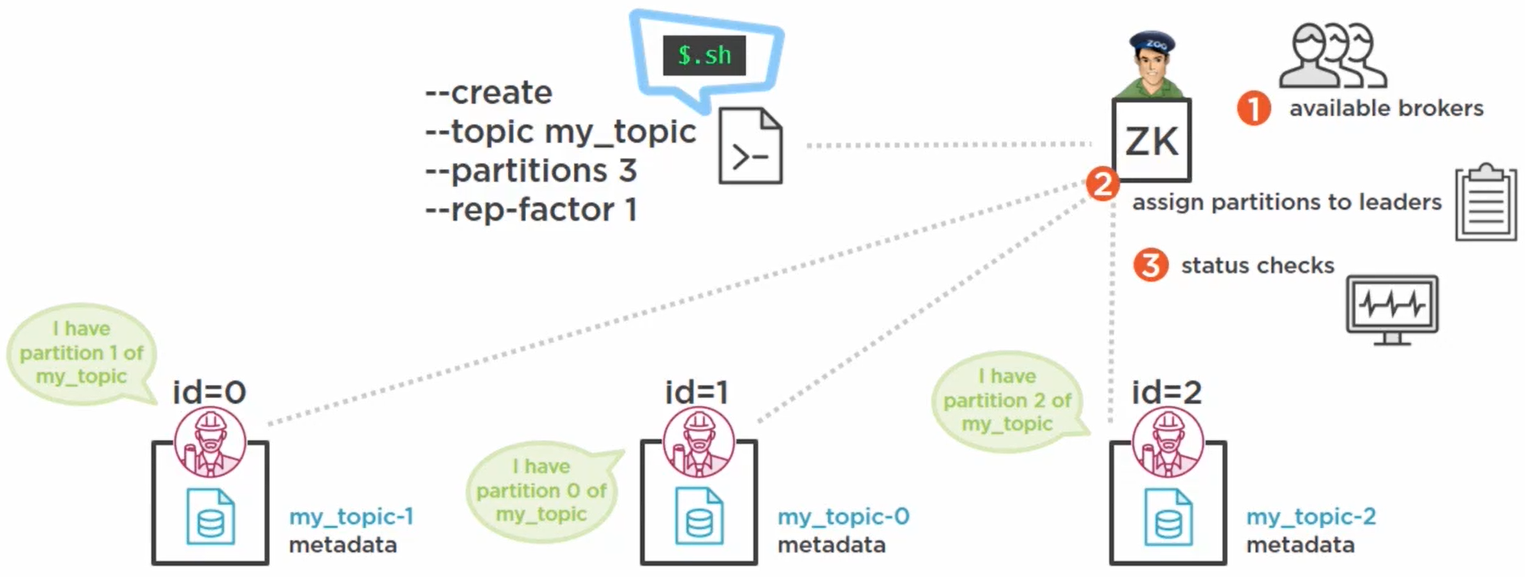
\includegraphics[width=10cm]{img/multiple_partitions.png}
		};
	\end{tikzpicture}
	\begin{itemize}
		\vspace{4cm}
		\item Le serveur Zookeeper (ZK) gère l'affectation des partitions aux brokers
		\item Dans l'exemple, il va choisir 3 brokers, un pour chaque partition
		\item Les brokers remontent les informations sur leur état à ZK
	\end{itemize}
\end{frame} 

\begin{frame}
	\frametitle{Producteur de messages vers les brokers}
	\begin{tikzpicture}[overlay,remember picture]
		\node[anchor=center,xshift=0pt,yshift=25pt]
		at (current page.center) {
			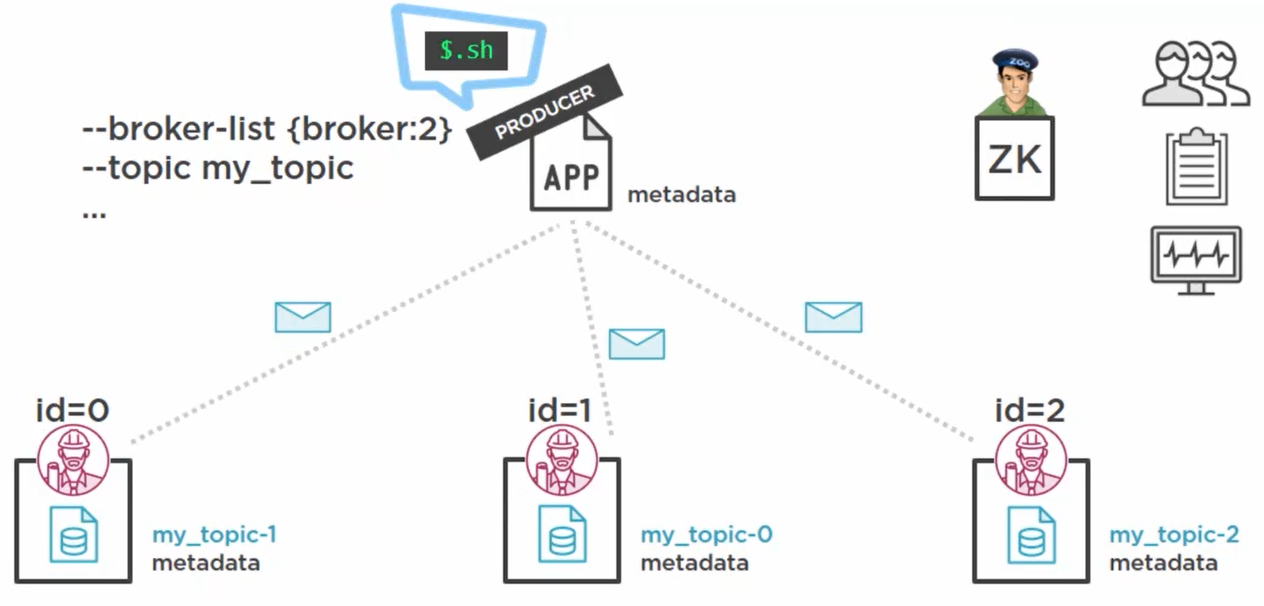
\includegraphics[width=10cm]{img/msg_producer_broker.png}
		};
	\end{tikzpicture}
	\begin{itemize}
		\vspace{4cm}
		\item Un producteur de messages peut connaître 1 seul broker (broker 2 ci-dessus)
		\item Ce broker indique au producteur quels autres brokers détiennent les autres partitions (transparent pour le dev)
		\item La production du message envoie le message à tous les brokers
	\end{itemize}
\end{frame} 

\begin{frame}
	\frametitle{Consommateur de messages depuis les brokers}
	\begin{tikzpicture}[overlay,remember picture]
		\node[anchor=center,xshift=0pt,yshift=25pt]
		at (current page.center) {
			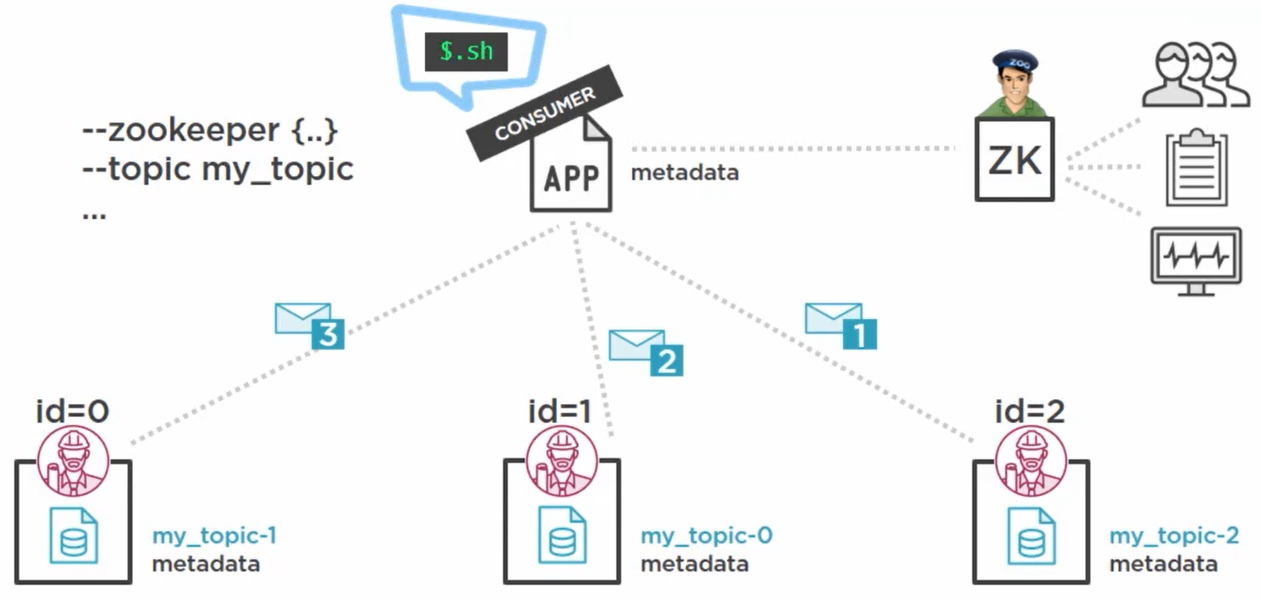
\includegraphics[width=10cm]{img/consumer_depuis_broker.png}
		};
	\end{tikzpicture}
	\begin{itemize}
		\vspace{4cm}
		\item Un consommateur collecte des méta-données depuis Zookeeper (liste et état des brokers)
		\item Il sollicite ensuite les différents brokers pour récupérer les messages
		\item Ces messages peuvent être ordonnés différemment sur chaque broker (le consommateur est responsable de gérer cela)
	\end{itemize}
\end{frame} 

\begin{frame}
	\frametitle{Compromis sur le nombre de partitions}
	\begin{itemize}
		\item Un nombre important de partitions a un impact négatif (surcharge) sur le Zookeeper (dans la coordination des brokers)
		\item Si l'on veut avoir un ordre total sur les messages, utiliser une seule partition par topic (sinon, ordres partiels / partition), ce qui peut être complexe à gérer dans certains cas
	\end{itemize}
\end{frame}

\begin{frame}
	\frametitle{Tolérance aux fautes (ou aux pannes)}
	\begin{tikzpicture}[overlay,remember picture]
		\node[anchor=center,xshift=0pt,yshift=25pt]
		at (current page.center) {
			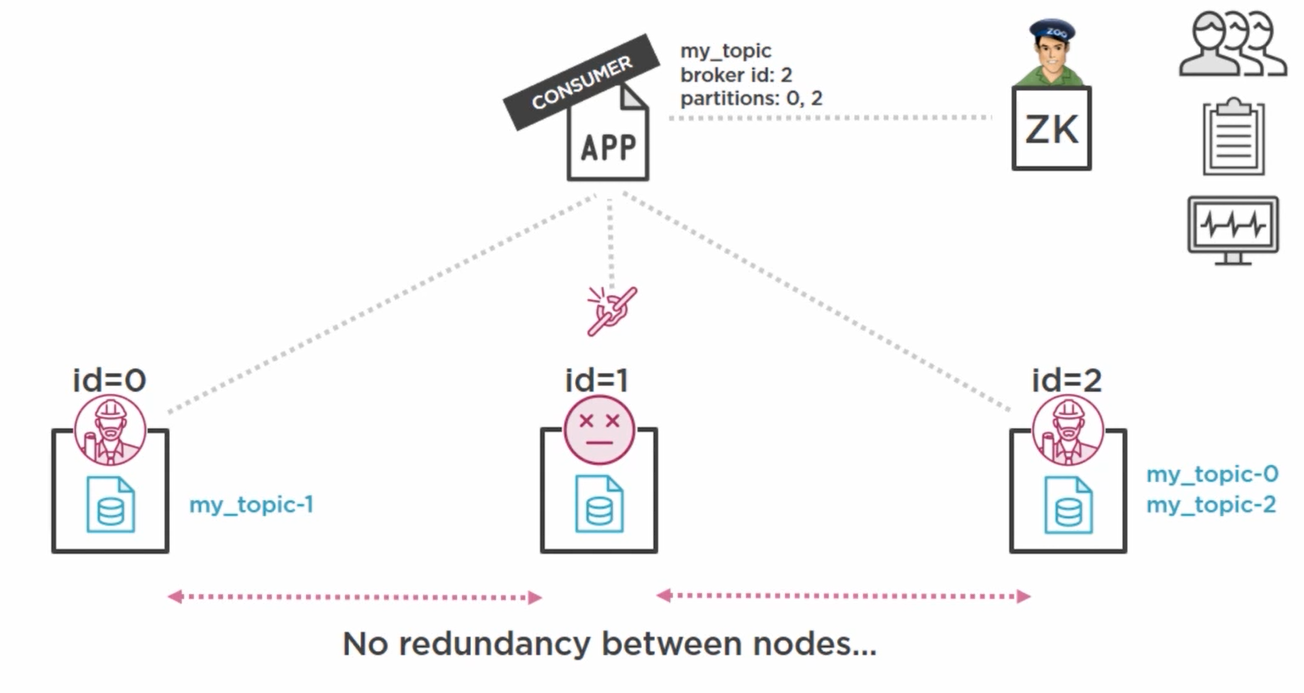
\includegraphics[width=9.2cm]{img/pannes_broker.png}
		};
	\end{tikzpicture}
	\begin{itemize}
		\vspace{4cm}
		\item Plusieurs fautes peuvent se produire (borker HS, coupure réseau, crash disque, ...)
		\item Le zookeeper gère l'inaccessibilité d'un broker pour informer les producteurs/consommateurs de messages (voir ci-haut)
		\item Mais les messages du broker en panne, qui n'ont pas été consommés, peuvent être perdus
	\end{itemize}
\end{frame} 

\begin{frame}
	\frametitle{Réplication pour tolérer les fautes/pannes}
		\begin{tikzpicture}[overlay,remember picture]
		\node[anchor=center,xshift=0pt,yshift=18pt]
		at (current page.center) {
			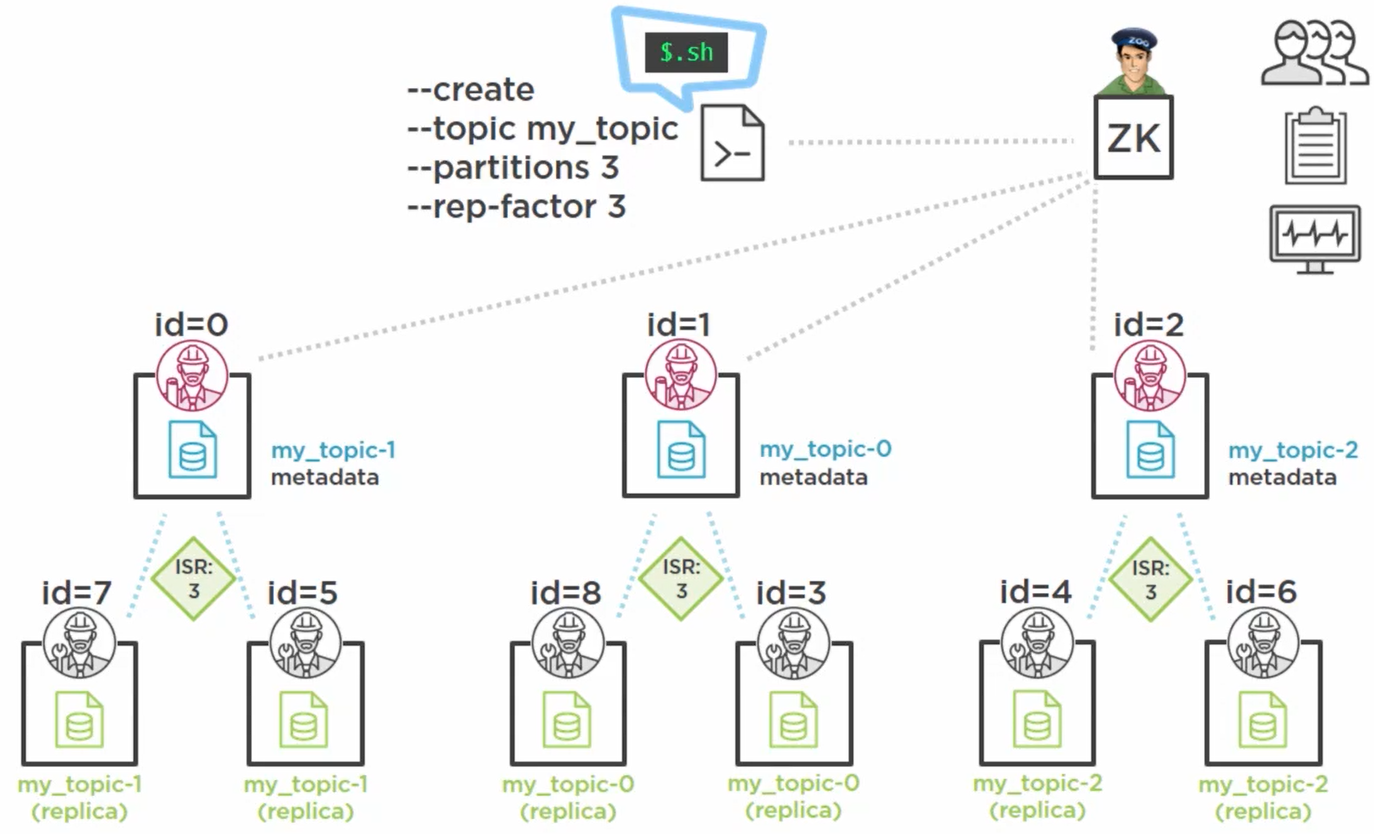
\includegraphics[width=9cm]{img/replication_factor.png}
		};
	\end{tikzpicture}
	\begin{itemize}
		\vspace{4.5cm}
		\item La tolérance aux fautes est atteinte par la réplication
		\item Le paramètre \texttt{replication-factor} permet d'indiquer le nombre de réplicats \textbf{par topic}
		\item Chaque broker (nommé leader) négocie avec d'autres brokers la gestion de la réplication
	\end{itemize}
\end{frame} 
	
\begin{frame}
	\frametitle{Réplication pour tolérer les fautes/pannes -suite-}
	\begin{tikzpicture}[overlay,remember picture]
		\node[anchor=center,xshift=0pt,yshift=20pt]
		at (current page.center) {
			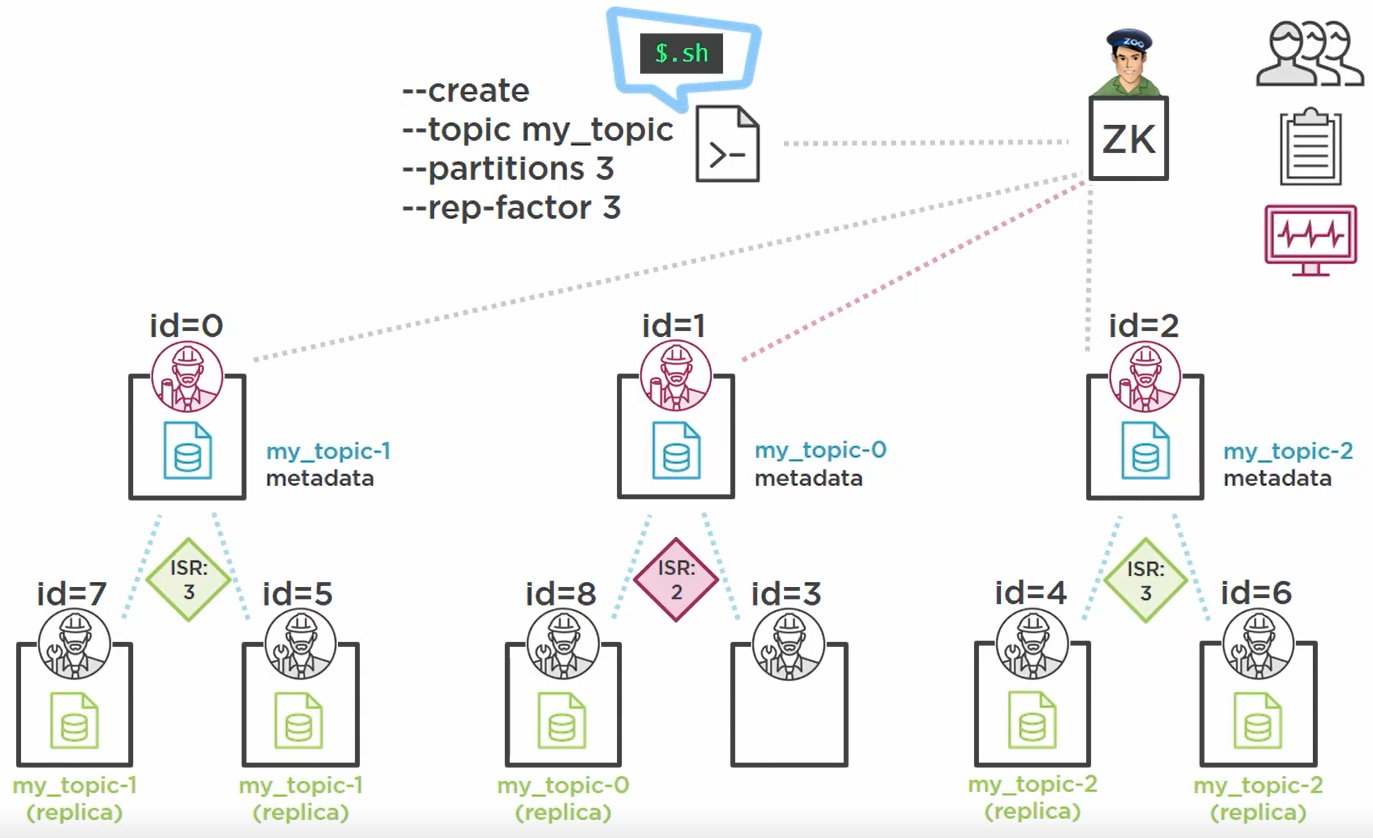
\includegraphics[width=8.5cm]{img/replication_isr.png}
		};
	\end{tikzpicture}
	\begin{itemize}
		\vspace{4.2cm}
		\item \texttt{isr} veut dire \textit{in-sync replicas}
		\item Tant que \texttt{isr} est égale à \texttt{replication-factor}, le cluster est considéré comme en bonne santé (\textit{healthy cluster})
		\item \texttt{isr} < \texttt{rep-factor} : Kafka continue de fonctionner mais ne fait pas de compensation
	\end{itemize}
\end{frame} 	

\begin{frame}
	\frametitle{A vos claviers}
	Tester la création d'un cluster de 3 brokers~: 
	\begin{itemize}
		\item 3 exécutions de kafka-server-start avec 3 fichiers server.properties distincts (à copier, renommer et éditer) server-0.properties, server-1.properties, ... avec~: 
		\begin{enumerate}
		 \item des id de brokers différents~: 0, 1 et 2
		 \item des dossiers différents pour les logs~: \texttt{/tmp/kafka-logs-0}, \texttt{/tmp/kafka-logs-1} ...
		 \item et des ports différents~: \texttt{<votre-hostname>:9092}, \texttt{<votre-hostname>:9093}, ...
		\end{enumerate}
		\item Créer un topic avec un facteur de réplication = 3~:\\
		\footnotesize
		\texttt{bin/kafka-topics.sh ---create ---topic replicated\_topic ---zookeeper <votre-hostname>:2181 ---replication-factor 3 ---partitions 1}
		\normalsize
	\end{itemize}
\end{frame} 	

\begin{frame}[fragile]
\frametitle{A vos claviers -suite-}
\begin{itemize}		
		\item Afficher les méta-données~: (option \texttt{---describe})\\
		\footnotesize
		\texttt{bin/kafka-topics.sh ---describe ---zookeeper <votre-hostname>:2181 ---topic replicated\_topic}
		\normalsize
		\item Ceci vous permet d'avoir~:
		
\begin{lstlisting}
Topic: replicated_topic 
 PartitionCount: 1 ReplicationFactor: 3 
 Configs:
  Topic: replicated_topic Partition: 0 Leader: 1 
                          Replicas: 1,0,2 Isr: 1,0,2    
\end{lstlisting}
\item Le leader de la réplication est le broker dont l'id est 1 (brokers 0 et 2 participent)
\item La ligne Topic aurait été affichée plusieurs fois si on avait plusieurs partitions
	\end{itemize}
On peut altérer les méta-données d'un topic existant avec l'option \texttt{---alter} (pour ajouter par ex la réplication à un cluster existant)
\end{frame} 

\begin{frame}[fragile]
	\frametitle{A vos claviers -suite-}
	\begin{itemize}		
		\item Créer un producteur de messages et produire quelques messages
		\item Créer un consommateur de messages
		\item Simuler une panne de l'un des brokers (le leader dont l'ID est 1), en tuant le processus de démarrage du broker (sur le terminal de démarrage de ce broker, faire un Ctrl-C ou un double Ctrl-C si vous êtes dans WSL sous Windows)
		\item Ré-exécuter la commande \texttt{---descibe} vue précédemment
		\item Que remarquez-vous dans le résultat affiché~?
		\item Le consommateur affiche une exception disant que le leader s'est arrêté, mais il continue de recevoir les messages		
		\item Produire un message pour le vérifier
		\item Redémarrer le broker arrêté. Il va rejoindre le cluster. Pour le vérifier exécuter la commande \texttt{---descibe}
	\end{itemize}
\end{frame} 

\section{Produire des messages}

\begin{frame}[fragile]
	\frametitle{Mettre en place l'environnement}
	\begin{itemize}
		\item Un cluster avec au moins un broker doit être démarré
		
		\item Ajouter la dépendance suivante à votre projet~:
\begin{lstlisting}
implementation group: 'org.springframework.kafka', name: 'spring-kafka', version: '2.7.8'
\end{lstlisting}
		\item Il faudra définir le paramètre de config. suivant~: (dans application.properties)
\begin{lstlisting}
spring.kafka.bootstrap-servers=<votre-hostname>:9092
\end{lstlisting}
	\item Si vous avez des difficultés à accéder au cluster Kafka depuis votre app (dans la suite du cours), voir ici comment on peut démarrer un cluster (ZK et Kafka) avec docker-compose~: \url{http://wurstmeister.github.io/kafka-docker/}
	\end{itemize}
\end{frame} 

\begin{frame}[fragile]
	\frametitle{Créer un topic Kafka}
Écrire une classe de création de topics~:

\begin{lstlisting}
@Configuration
class KafkaTopicConfig {	
	@Bean
	public NewTopic topic1() {
		return TopicBuilder.name("mytopic-1").build();
	}
	@Bean
	public NewTopic topic2() {
		return TopicBuilder.name("mytopic-2").build();
	}
	...
}
\end{lstlisting}
	
On peut affiner la création de topics en indiquant, par ex, une période de rétention des messages (en millisecondes)~:\\
\footnotesize
\texttt{<...>.config(TopicConfig.RETENTION\_MS\_CONFIG, "1680000").build();}
\normalsize
\end{frame} 

\begin{frame}[fragile]
	\frametitle{Envoyer un message}
\begin{lstlisting}
@Component
class KafkaSenderExample {	
	private KafkaTemplate<String, String> kafkaTemplate;	
	@Autowired
	KafkaSenderExample(KafkaTemplate<String, String> kafkaTemplate) {
		this.kafkaTemplate = kafkaTemplate;
	}	
	void sendMessage(String message, String topicName) {
		kafkaTemplate.send(topicName, message);
	}
}
\end{lstlisting}
	\begin{itemize}
		\item Ici on utilise un String (De-)Serializer pour les clés/valeurs des messages (voir paramètres de \texttt{KafkaTemplate})
		\item Ignorer le warning d'IntelliJ sur {\footnotesize \texttt{KafkaTemplate<String, String>}}
		\item Il est possible d'avoir un autre (de-)serializer pour JSON par ex~:\\
		\scriptsize
		\url{https://howtodoinjava.com/kafka/spring-boot-jsonserializer-example/}
		\normalsize
	\end{itemize}
\end{frame} 

\begin{frame}[fragile]
	\frametitle{Autres paramètres pour l'envoi de messages}
	\begin{itemize}
		\item L'objet \texttt{kafkaTemplate} a été utilisé dans cet exemple pour envoyer un message (une valeur, sans clé) à un topic
		\item Cet objet permet également d'envoyer des paires clés-valeurs plutôt que des valeurs seules (recommandé)
		\item Il permet aussi d'envoyer un message à une partition en particulier
		\item Plus généralement, on peut passer en paramètre un objet \texttt{ProducerRecord} (objet de base d'Apache Kafka, enveloppé par \texttt{kafkaTemplate} de Spring Kafka), qu'on peut paramétrer assez finement
		\item Plusieurs méthodes \texttt{send(...)} offertes par cet objet
	\end{itemize}
\end{frame} 

\begin{frame}[fragile]
	\frametitle{Processus d'envoi de message -- Partie 1}
	\begin{tikzpicture}[overlay,remember picture]
		\node[anchor=center,xshift=0pt,yshift=20pt]
		at (current page.center) {
			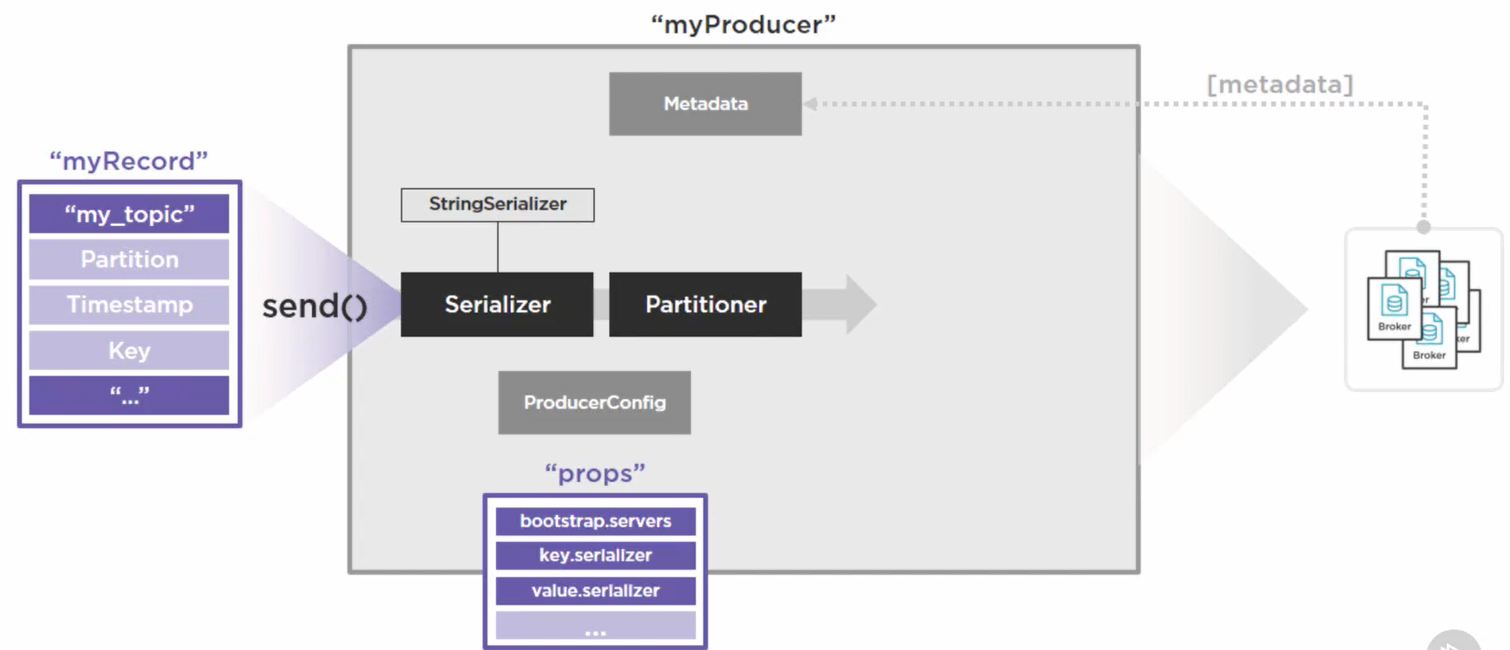
\includegraphics[width=12cm]{img/process_msg_sending_1.png}
		};
	\end{tikzpicture}
	\begin{itemize}
		\vspace{4cm}
		\item L'envoi de messages est gérée par un objet \texttt{KafkaProducer}
		\item Cet objet va gérer la serialisation (vers String dans l'exemple) puis le routage vers les partitions
	\end{itemize}
\end{frame} 

\begin{frame}[fragile]
	\frametitle{Routage vers les partitions}
	\begin{tikzpicture}[overlay,remember picture]
		\node[anchor=center,xshift=0pt,yshift=0pt]
		at (current page.center) {
			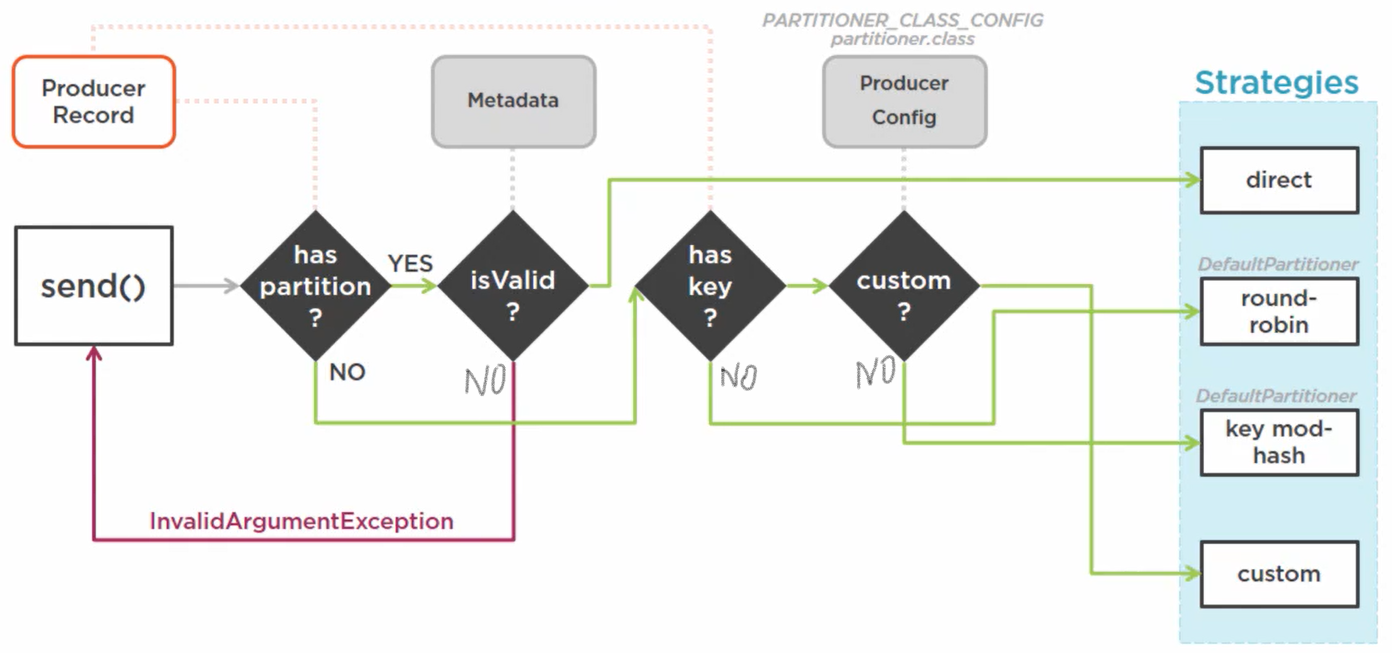
\includegraphics[width=12cm]{img/routing_to_partitions.png}
		};
	\end{tikzpicture}
	
	\begin{itemize}
		\vspace{4cm}
		\item 4 stratégies de routages possibles (voir à droite)
		\item De la plus simple (sans routage) au routage personnalisé défini dans une classe utilisateur
	\end{itemize}
\end{frame} 

\begin{frame}[fragile]
	\frametitle{Processus d'envoi de message -- Partie 2}
	\begin{tikzpicture}[overlay,remember picture]
		\node[anchor=center,xshift=0pt,yshift=20pt]
		at (current page.center) {
			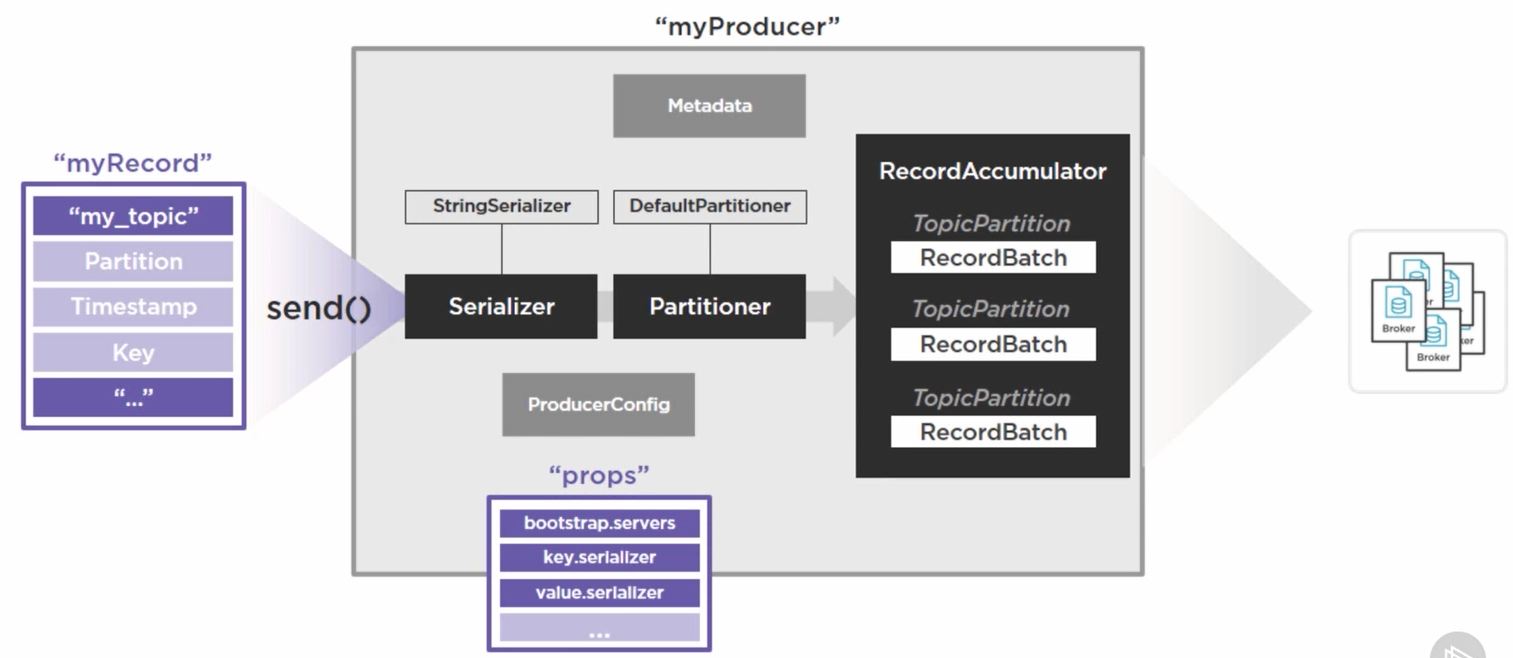
\includegraphics[width=12cm]{img/process_msg_sending_2.png}
		};
	\end{tikzpicture}
	\begin{itemize}
		\vspace{4cm}
		\item Dernière phase dans l'envoi de message est la bufferisation
		\item Plusieurs stratégies possibles (paramétrables) pour créer des batchs (cumuler plusieurs messages et faire un seul envoi, selon des contraintes de taille, de temps, ...)
	\end{itemize}
\end{frame}

\begin{frame}[fragile]
	\frametitle{Garanties d'envoi}
	\begin{itemize}
		\item Il est possible d'indiquer des niveaux d'accusé de réception (\texttt{acks})~:
		\begin{itemize}
			\item 0 : envoyer et oublier le message
			\item 1 : accusé de réception du leader seulement
			\item 2 : tous les \texttt{isr} doivent envoyer un accusé de réception
		\end{itemize}
	\item Il est possible également de faire des reprises d'envoi de messages (\textit{retry}) et/ou forcer la reprise de l'envoi dans l'ordre (pas d'envoi d'un 2nd message tant que le 1er n'a pas réussi)
	\item Tout cela est paramétrable dans la configuration du \textit{Producer}
	\end{itemize}
\end{frame} 

\begin{frame}
	\frametitle{A vos claviers}
	\begin{itemize}
		\item Reprendre votre application Spring Boot et produire un message comportant le username et sa localisation, vers un topic dédié, non partitionné et répliqué avec un facteur de 3
		\item Utiliser un serializer String ("<username>:<localisation>") au début et ensuite un serializer JSON
		\item Vérifier la bonne réception des messages dans un consommateur lancé depuis le terminal, comme fait précédemment
	\end{itemize}
\end{frame}

\section{Consommer des messages}

\begin{frame}
	\frametitle{Même environnement que le producteur}
	\begin{itemize}
		\item On utilise les mêmes paramètres que dans le producer (dans \texttt{application.properties})~:
		\texttt{bootstrap-servers}, ...
		\item La classe de base est KafkaConsumer qui permet à un objet de souscrire (\textit{subscribe}) aux événements de réception de message
		\item Avec Spring MVC, c'est encore plus simple~: une méthode ou une classe annotée \texttt{@KafkaListener}
	\end{itemize}
\end{frame} 

\begin{frame}[fragile]
	\frametitle{Exemple de consommateur de messages}
\begin{lstlisting}
@Component
class KafkaListenerExample {
	Logger LOG = LoggerFactory.getLogger(KafkaListenerExample.class);
	@KafkaListener(topics = "my_topic")
	void listener(String data) {
		LOG.info(data);
	}
}
\end{lstlisting}
\begin{itemize}
	\item Ici, on a une méthode qui est annotée par \texttt{@KafkaListener}
	\item Dans l'annotation, on ajoute le topic (ou les topics, séparés par virgules) au(x)quel(s) souscrit ce consommateur
	\item A la réception d'un message sur ce topic, la méthode est exécutée
\end{itemize}
\end{frame} 

\begin{frame}[fragile]
	\frametitle{Un consommateur de messages selon leur type}
\begin{lstlisting}
@Component
@KafkaListener(id = "class-level", topics = "my_topic")
class KafkaClassListener {
	@KafkaHandler
	void listen(String message) {
		LOG.info("KafkaHandler[String] {}", message);
	}
	@KafkaHandler(isDefault = true)
	void listenDefault(Object object) {
		LOG.info("KafkaHandler[Default] {}", object);
	}
}
\end{lstlisting}
	\begin{itemize}
		\item Ici, la méthode à exécuter est celle qui correspond au type spécifique du message reçu
		\item Si aucune méthode ne correspond au type de message reçu, celle marquée \texttt{isDefault} est exécutée
	\end{itemize}
\end{frame} 

\begin{frame}[fragile]
	\frametitle{Un consommateur avec plus de paramètres}
\begin{lstlisting}
@KafkaListener(
  groupId = "my_topic",
  topicPartitions = @TopicPartition(
    topic = "my_topic",
    partitionOffsets = { @PartitionOffset(
	  partition = "0",
	  initialOffset = "0") }))
void listenToPartitionWithOffset(
  @Payload String message,
  @Header(KafkaHeaders.RECEIVED_PARTITION_ID) int partition,
  @Header(KafkaHeaders.OFFSET) int offset) {
	LOG.info("Received message [{}] from partition-{} with offset-{}",
	message,
	partition,
	offset);
}
\end{lstlisting}
On verra la notion de groupe plus tard
\end{frame} 

\begin{frame}[fragile]
	\frametitle{Exemple précédent}
	\begin{itemize}
		\item Dans l'exemple précédent, on a indiqué \texttt{initialOffset = "0"}
		\item Cela veut dire que le consommateur veut récupérer tous les messages depuis le début de la création de la partition (à chaque redémarrage de l'application)
		\item On a également utilisé l'annotation @Header qui a permis d'accéder à un certain nombre d'informations utiles~: l'id de la partition et l'offset du message courant

	\end{itemize}
\end{frame} 

\begin{frame}[fragile]
	\frametitle{Pour tester un consommateur avec une production ``massive" de messages}
	\begin{itemize}
		\item Il existe un script qui vient avec Kafka et qui permet de produire une grande quantité de messages
		\item Celui-ci permet de tester les performances de la configuration
		\item Exécuter la commande~:
\begin{lstlisting}
bin/kafka-producer-perf-test.sh ---topic my_topic ---num-records 50 ---record-size 1 ---throughput 10 ---producer-props bootstrap.servers=<votre-hostname>:9092
\end{lstlisting}
Cette commande indique le topic cible, le nombre de messages (50), la taille des messages (1 octet), le débit (10 messages par seconde) et le broker
\item A tester sur votre installation
	\end{itemize}
\end{frame} 

\begin{frame}[fragile]
	\frametitle{Ce qui se cache derrière un consommateur}
	\begin{tikzpicture}[overlay,remember picture]
		\node[anchor=center,xshift=0pt,yshift=30pt]
		at (current page.center) {
			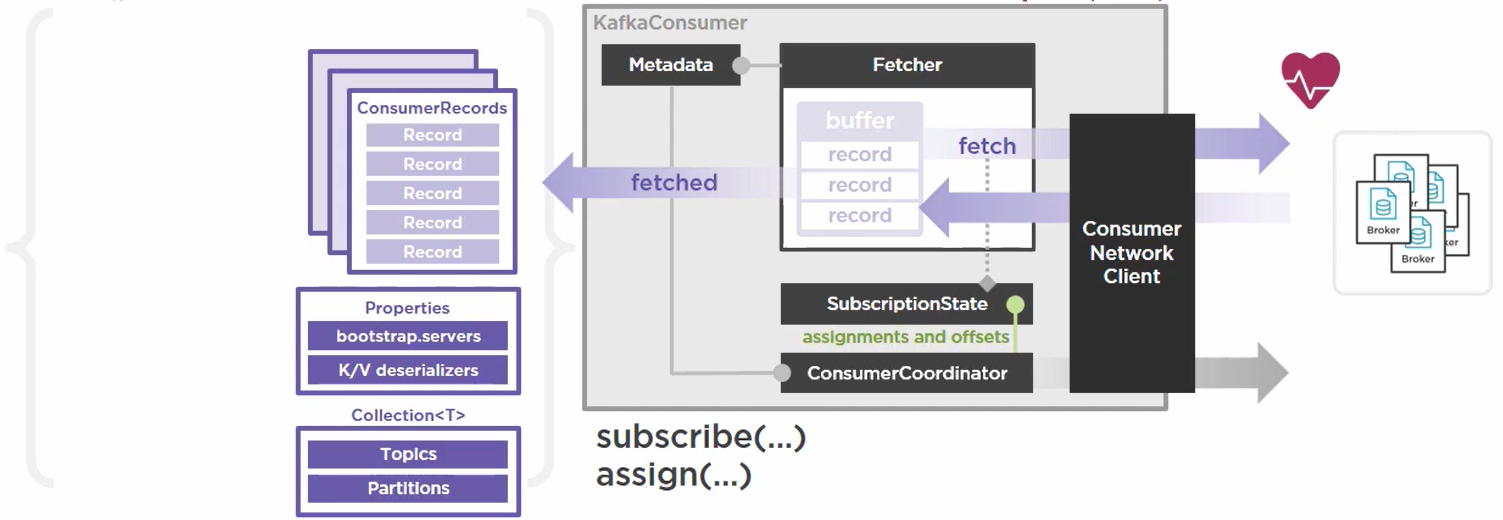
\includegraphics[width=11cm]{img/consumer_internals.png}
		};
	\end{tikzpicture}
	\begin{itemize}
		\vspace{3.5cm}
		\item L'objet au coeur des interactions avec le cluster est un objet de type \texttt{KafkaConsumer} (au centre de la figure)
		\item Celui-ci gère les méta-données, la souscription à des topics ou l'affectation (assign()) à des partitions de topics
		\item Il fait des polls périodiques (fréquence paramétrable) et bufferise les messages avant de les retourner au consommateur sous forme d'objets \texttt{ConsumerRecord}
	\end{itemize}
\end{frame} 

\begin{frame}[fragile]
	\frametitle{Retour sur les offsets}
	\begin{itemize}
		\item Un offset existe par partition et par consommateur
		\item Un message lu ne veut pas dire qu'il est est validé (commit de son offset au broker). Il se peut que le consommateur tombe en panne pendant le traitement du message
		\item Par défaut, le consommateur fait un auto-commit (paramètre par défaut = true), lors de la lecture d'un message et après une durée de 5000 ms (paramètre par défaut), il envoie son dernier offset
	\end{itemize}
\end{frame} 

\begin{frame}[fragile]
\frametitle{Retour sur les offsets -suite-}
%	\begin{tikzpicture}[overlay,remember picture]
%		\node[anchor=center,xshift=0pt,yshift=35pt]
%		at (current page.center) {
%			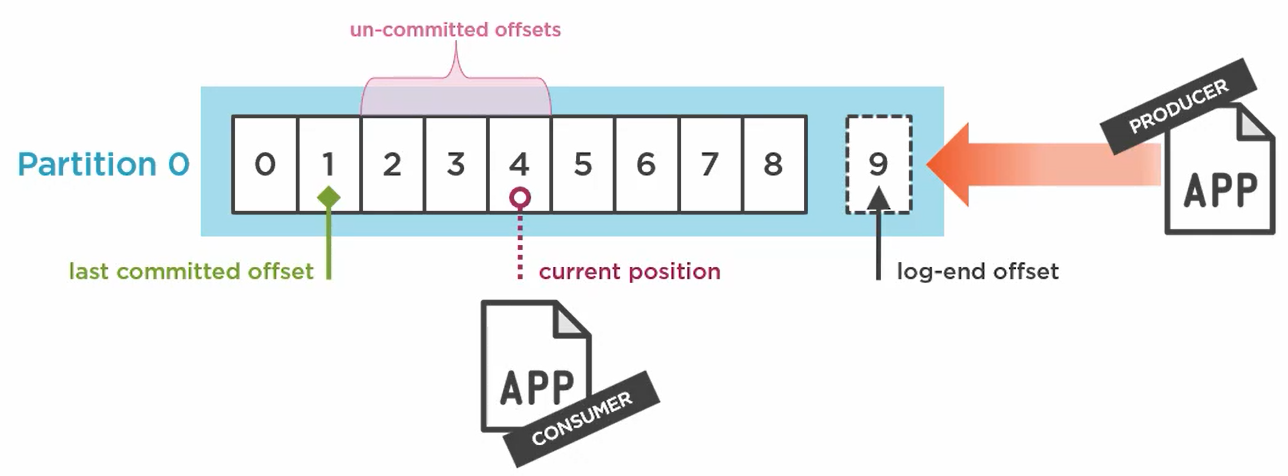
\includegraphics[width=11cm]{img/last_offset.png}
%		};
%	\end{tikzpicture}
\begin{itemize}		
		\item Il est possible de fixer la valeur de l'auto-commit à false. Dans application.properties~:
\begin{lstlisting}
enable.auto.commit=false
spring.kafka.listener.ack-mode=manual
\end{lstlisting}
		et ensuite faire des commits manuels pour éviter la perte de messages en cas de pannes~:
	\begin{itemize}		
		\item Ajouter un paramètre au listener~:\\ \texttt{Acknowledgment acknowledgment}
		\item Faire un commit~: \texttt{acknowledgment.acknowledge();}
	\end{itemize}
\item Les offsets sont gérés par Kafka dans un topic à part nommé \texttt{\_\_consumer\_offsets}
	\end{itemize}
\end{frame} 

\begin{frame}[fragile]
	\frametitle{Particularités des consommateurs}
	\begin{itemize}
		\item Un consommateur donné effectue un poll dans un seul thread
		\item Si l'on fait un traitement lourd sur un message consommé, ceci n'a pas d'impact sur les autres composants du système (le cluster, les autres consommateurs ou les producteurs)
		\item Mais en pratique, il vaut mieux gérer les consommateurs par \textbf{groupe} pour se répartir la charge de consommation de messages
		\item C'est la solution de Kafka pour rendre les consommateurs scalables
	\end{itemize}
\end{frame} 

\begin{frame}[fragile]
	\frametitle{Groupe de consommateurs}
	\begin{itemize}
		\item Collection de consommateurs travaillant en équipe
		\item Pour qu'un consommateur puisse appartenir à un groupe, il faut définir le paramètre \texttt{groupId}
		\item Ils partagent la charge de consommation des messages
		\item \textbf{Une partition} est affectée à un consommateur d'un groupe
		\item S'il y a plus de consommateurs (d'un même groupe) que de partitions, les consommateurs en trop sont libres
		\item Dès qu'il y a une nouvelle partition qui se crée, elle est affectée au consommateur libre (\textit{rebalancing})
		\item Le \textit{rebalancing} est fait aussi lorsque l'un des consommateur est arrêté pour attribuer sa/ses partition(s) aux autres consommateurs du groupe
	\end{itemize}
\end{frame} 

\begin{frame}[fragile]
	\frametitle{Groupe de consommateurs -suite-}
	\begin{itemize}
		\item Pour déclarer l'appartenance à un groupe, il suffit d'ajouter un \textit{groupId} à un consommateur~:
	\end{itemize}
\begin{lstlisting}
@KafkaListener(topics = "my_topic", groupId = "my-topic")
void listenToPartitionWithOffset2(
  ConsumerRecord<String,String> record,
  Acknowledgment acknowledgment) {
	LOG.info("Listener 2 - Received message [{}] from partition-{} with offset-{} recorded at: {}",
	record.value(),
	record.partition(),
	record.offset(),
	new Date(record.timestamp()));
	acknowledgment.acknowledge();
}
\end{lstlisting}
Noter la récupération du timestamp ci-dessus
\end{frame} 

\begin{frame}[fragile]
	\frametitle{Groupe de consommateurs -suite-}
	\begin{itemize}
		\item Tester un groupe de consommateurs sur un topic à 3 partitions et observer quel consommateur/listener consomme les messages de quelle partition
		\begin{itemize}
			\item Altérer le topic existant pour mettre en place de nouvelles partitions, si vous avez un topic à une partition~:
			\footnotesize
			\texttt{bin/kafka-topics.sh ---alter ---zookeeper localhost:2181 ---topic my\_topic ---partitions 3}
			\normalsize
		\end{itemize}
		\item Ajouter deux autres consommateurs et observez ce qui se passe
		\item Y a-t-il un consommateur (en trop) qui ne consomme rien~?		
		\item Réduire le nombre de consommateurs à 2. A qui sont attribuées 2 partitions~?
	\end{itemize}
Faire cela sans arrêter Zookeeper ou vos brokers. Exécuter les commandes dans un nouveau terminal, et modifier/ré-exécuter votre app Spring
\end{frame} 

\section{Conclusion}
\begin{frame}
	\frametitle{\textit{Wrap-up}}
	\begin{itemize}
		\item Kafka : un système distribué de gestion de messages à grand débit selon le modèle publish/subscribe
		\item On a vu comment mettre en place les trois composants de ce système~: le cluster, les producteurs de messages et les consommateurs (avec Spring Kafka pour les deux derniers)
		\item De nombreux sujets n'ont pas été abordés ici : paramétrage fin du système (timeouts, délais, tailles des buffers, ...), contrôler les déplacements/flux de contrôle (seek(), pause(), resume(), ...), \textit{Rebalance Listeners}, ..
		\item Plein de projets dans l'écosystème Kafka~: \textit{Schema Registry} (harmoniser les schémas de données et leur (dé-)serialisation), \textit{Kafka Connect/Hub} (gérer l'hétérogénéité des sources/cibles de données), \textit{Kafka Streams}, ... (chez confluent.io notamment)
	\end{itemize}
\end{frame}
\begin{frame}
	\frametitle{Références bibliographiques}

	\begin{itemize}				
		\item Site web Apache Kafka~:\\
		\url{https://kafka.apache.org/}
		\item Site web spring.io~:\\
		\url{https://docs.spring.io/spring-kafka/docs/current/reference/html/}
		
		\item Tutos sur Pluralsight et Baeldung
	\end{itemize}
\end{frame}


\begin{frame}
	\begin{tikzpicture}[overlay,remember picture]
		\node[anchor=center,xshift=0pt,yshift=0pt]
		at (current page.center) {
			
\includegraphics[width=4cm]{img/question.jpg}
		};
	\end{tikzpicture}
\end{frame}

\end{document}
